\chapter{実験}

本実験の概要を図\ref{fig:enquete}に示す.
本実験では,まず物語文を元に各感情を指定した音声データを生成し,Webのアンケートシステムを用いて複数の被験者に評価してもらい,学習データを作成する.
その後,学習データを用い交差検証を行う.

\begin{figure}[ht]
  \begin{center}
    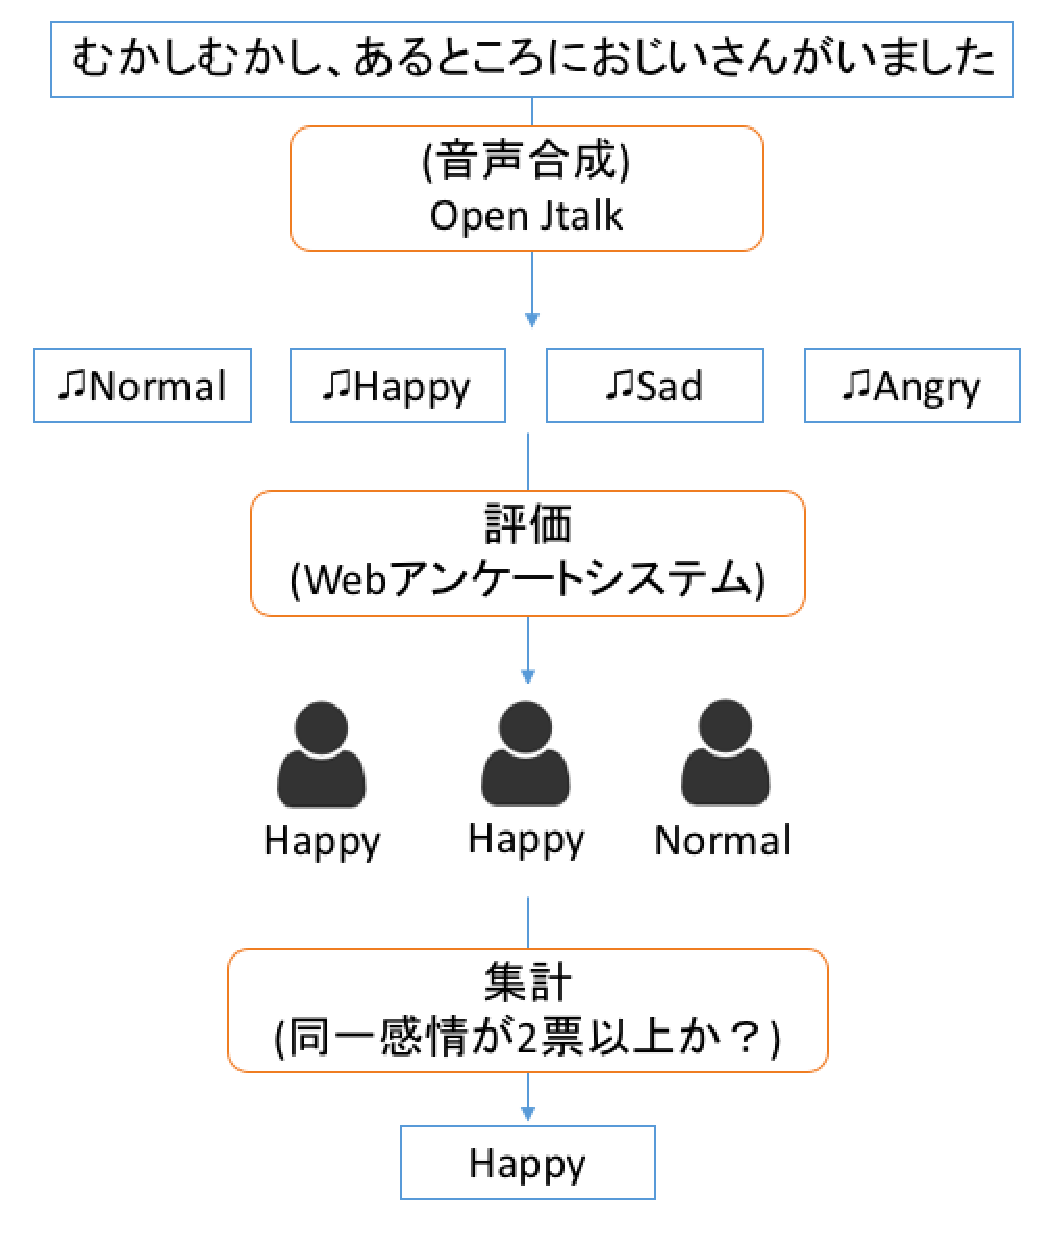
\includegraphics[clip,width=7.0cm]{fig/enquete.eps}
    \caption{学習データの作成手順}
    \label{fig:enquete}
  \end{center}
\end{figure}

\subsection{データの作成}
提案手法で述べた通り物語データを文に区切り,一文につきそれぞれ4種類の感情を指定して音声データを生成する.

本実験では物語データとして,青空文庫\cite{aozora}にある5つの物語を用いる.
今回は文体を近づけるために同じ訳者の童話を中心に「白雪姫」,「赤ずきんちゃん」,「浦島太郎」,「ジャックと豆の木」,「ヘンゼルとグレーテル」を用いた.
なお,ルビのデータが含まれているため予めタグを除いておく.

本研究の音声合成にはオープンソフトのOpen JTalk\cite{jtalk}を用いる.
Open JTalk は形態素解析部に MeCab\cite{mecab},発音辞書に NAIST Japanese Dictienary\cite{naist}を用いてる.
波形生成部にはMMDAgent\cite{mei}にあるMeiのサンプルを用いてる.
NOMAL,HAPPY,ANGRY, BASHFUL,SADの5種類のサンプルがあるが,先行研究に従いこの内のBASHFULを除いた4種類を用いた.
なお,音声データはWAVE形式として保存される.

\subsection{学習データの収集}
\begin{figure}[ht]
  \begin{center}
    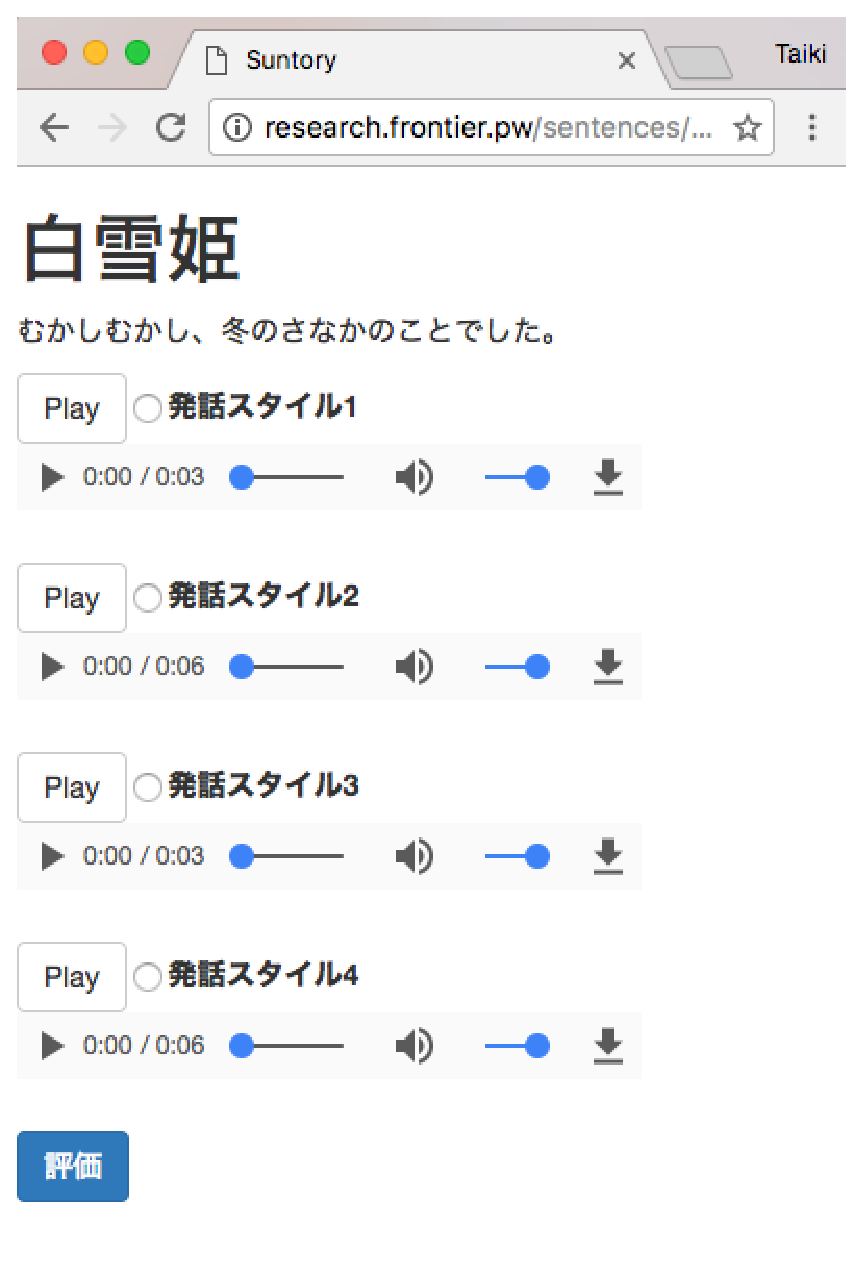
\includegraphics[clip,width=7.0cm]{fig/web.eps}
    \caption{WEBアンケートシステム画面}
    \label{fig:web}
  \end{center}
\end{figure}

Web上で学習データを収集するためのシステムを構築した.
そのシステム画面を図\ref{fig:web}に示す.
被験者には文ごとに各感情のパラメタで合成した音声をそれぞれ聞いてもらい内容にもっとも適切(自然)であると思われる感情を1つだけ選択してもらう.
しかし,感情は主観的な尺度であるため一人だけの評価では信頼性が低い.
そこで,一文に対して同じ感情の評価が二票集まった時点で,その文の感情を決定することとした.
したがって,同じ感情の評価が二票あるまで他の被験者に評価し続けてもらう.
被験者等に関する詳細を表\ref{enviroment}に示す.

\begin{table}[ht]
  \begin{center}
  \caption{学習データの収集}
  \label{enviroment}
  \begin{tabular}{|c|l|}
    \hline
    被験者 & 東京理科大学の学部生及び大学院生 \\ \hline
    人数 & 学部生15名,大学院生2名 \\ \hline
    取得期間 & 2017年1月9日〜25日 \\ \hline
    評価取得数 & 2641 \\ \hline
  \end{tabular}
  \end{center}
\end{table}

\subsection{評価}
本実験では,leave-one-out交差検証を行い,判定結果に対応する入力データの集合をTP,FP,TN,FNを次のように定義する.

\begin{description}
   \item[True Positive(TP)] 実際の感情のものを実際の感情であると予測したものの件数
   \item[True Negative(TN)] 実際の感情でないものをその感情でないと予測したものの件数
   \item[False Positive(FP)] 実際の感情でないものを実際の感情であると予測したものの件数
   \item[False Negative(FN)] 実際の感情のものを実際の感情でないと予測したものの件数
 \end{description}


以上をふまえ,分類器の性能評価を式(1),(2),(3),(4)で行う.
本研究は分類推定を目的としているため特にF値(4)に注目する.

\begin{eqnarray}
  正解率(Ac) =  \frac{TP + TN} {TP + TF + NP + NF}
\end{eqnarray}

\begin{eqnarray}
  適合率(Pr) = \frac{TP} {TP + FP}
\end{eqnarray}

\begin{eqnarray}
  再現率(Re) =  \frac{TP} {TP + FN}
\end{eqnarray}

\begin{eqnarray}
  F値 =  \frac{2*Pr*Re}{Pr + Re}
\end{eqnarray}


\subsection{比較実験}
提案手法の有効性を検証するために,同様な実験をセリフ文のみに絞った場合とさらに機能語に絞らなかった場合とそれぞれ行った.
さらに,ランダムフォレストの比較としてSVMを用いた実験も行った.
このとき,ランダムフォレストと同様にSVMでもグリットサーチで最適なパラメタを導出した.
